\documentclass[../../main.tex]{subfiles}

\begin{document}
\chapter{Relations between Variables}
Marcus starts with the following observation:

\begin{observation}
    The human brain is capable of performing operations like addition, multiplication, inflecting verbs, and so on.
\end{observation}

What do all these algebraic operations have in common? They all operate on variables based on rules. Thus, Marcus calls them \emph{relations between variables}.

\section{UQOTOM}
Instead of considering all these functions of human cognition at once, Marcus focusses on a very special subclass of operations. He refers to them as \emph{UQOTOM}, which stands for \emph{universally quantified one-to-one mapping}. Like the name suggests, they are defined as follows:

\begin{definition}[UQOTOM]
    A mapping $f: X \to Y$ is a UQOTOM if it is \emph{one-to-one} and \emph{universally quantified}. Universally quantified specifies that $f$ is defined for all $x \in X$, i.e. that $f$ is a valid function in the mathematical sense.
\end{definition}

Some important examples of UQOTOMs that Marcus is going to analyze are the identity function, and the simple past operation with produces the simple past of a verb. According to Marcus:

\begin{citecallout}[\textcite{marcus_algebraic_mind}]
    I do not mean to suggest that UQOTOM are the only mappings
    people compute. But UQOTOM are especially important to the arguments that follow because they are functions in which every new input has a new output. Because free generalization of UQOTOM would
    preclude memorization, evidence that people (or other organisms) can
    freely generalize UQOTOM would be particularly strong evidence in
    support of the thesis that people (or other organisms) can perform operations over variables.
\end{citecallout}

Based on this quote, we can see that Marcus is interested in UQOTOMs because they enforce a system to \emph{generalize} mappings. That is, given a never-before-seen input, a potential model implementing this UQOTOM must produce a new output that has not been produced before. And this generalization is a central aspect of \emph{symbol manipulation} according to Marcus.

\begin{citecallout}[\textcite{marcus_algebraic_mind}]
    To a system that can make use of algebralike operations over variables,
    free generalization comes naturally.
\end{citecallout}

Furthermore, he specifies algebraic rules further and he writes:

\begin{citecallout}[\textcite{marcus_algebraic_mind}]
    Algebraic rules are not finite tables of memorized facts or relationships between specific instances but open-ended relationships that can be freely generalized to all elements within some class.
\end{citecallout}

Most decisively, for Marcus, a UQOTOM isn't just a special type of function; it is the very implementation of an algebraic rule. He writes:

\begin{citecallout}[\textcite{marcus_algebraic_mind}]
    When such a network represents identity or some other UQOTOM,
    it represents an abstract relationship between variables—which is to say
    that such a network implements an algebraic rule.
\end{citecallout}

\begin{critique}
    The implication
    \[
        f \text{ is a UQOTOM} \implies f \text{ implements an algebraic rule}
    \]
    is too simple and doesn't grasp the complexity of algebraic rules. It is also not a suitable indicator for whether a model implements algebraic rules. For example, the function $f(x) = x^2$ is not a UQOTOM, but it is an algebraic rule. The fundamental flaw is that one cannot reduce the analysis of algebraic rules to the analysis of UQOTOMs.
\end{critique}

\subsection{Humans can freely generalize UQOTOMs}
Now that Marcus has established his framework of UQOTOMs, he argues that humans can freely generalize these UQOTOMs. He provides evidence for this claim with the following example:

\begin{example}
    When you are presented the pattern
        \begin{table}[h]
        \centering
        \begin{tabular}{c|c}
            Input & Output \\
            \hline
            1010 & 1010 \\
            0100 & 0100 \\
            1110 & 1110 \\
            0000 & 0000 \\
            1111 & ? \\
        \end{tabular}
    \end{table}
    and asked to predict the output of 1111, what would you answer?
\end{example}

Marcus argues that most people would answer 1111, because humans have a bias for generalizing UQOTOMs, which is why the identity mapping is generalized in this example. He concludes:

\begin{premise}
    Humans can freely generalize UQOTOMs.
\end{premise}

%TODO: quote; use another premise subclass of algebraic rules is UQOTOM -> model should generalize UQOTOMs

\subsection{Multilayer Perceptrons and Operations over Variables}
Next, Marcus emphasizes the distinction between models that allocate \emph{one node per variable}, and models which allocate \emph{multiple nodes per variable}:

\begin{definition}
    A model is said to allocate \emph{one node per variable} if it has a single node for each variable in the input. A model is said to allocate \emph{multiple nodes per variable} if it has multiple nodes for each variable in the input.
\end{definition}

\begin{citecallout}[\textcite{marcus_algebraic_mind}]
    Again, what is relevant here is not the sheer number of input units
    but rather the number of input units allocated to representing each input
    variable.
\end{citecallout}

\begin{critique}
    In the mathematical setting of neural networks that represent one-to-one mappings, it makes no difference whether, say, 5 input nodes all together represent a single variable, or five individual variables all encoded by a single node each. Furthermore, he also does not apply this framework, or only very vaguely, as we will see in the next section.
\end{critique}

Additionally, he points out that this distinction is not to be confused with \emph{localist} and \emph{distributed} representations:

\begin{citecallout}[\textcite{marcus_algebraic_mind}]
    While all models that use distributed representations allocate more than one variable per node, it is
    not the case that all localist models allocate a single node per variable.
\end{citecallout}

With this definition established, Marcus claims that:

\begin{citecallout}[\textcite{marcus_algebraic_mind}]
    One-node-per-variable models, it turns out, can and indeed (the caveats in note 5 notwithstanding) must represent universally
    quantified one-to-one mappings.
\end{citecallout}

\begin{critique}
    Again, he assumes the network to only have one input node, which is not the same as having one node per variable. Furthermore, in note 5 he explains that he assumes the network to only have linear activation functions. Such a network must learn a linear mapping, and every mapping $f(x) = \alpha \cdot x$ is one-to-one for $\alpha \neq 0$.

    Note that if we had multiple input nodes instead, a linear mapping is described by a matrix multiplication $f(\bm{x}) = A \cdot \bm{x}$. In this case, the mapping is one-to-one if and only if $A$ is invertible, which is not guaranteed for all matrices.
\end{critique}

\begin{critique}
    This described case of a single input node with linear activation functions is very specific and doesn't serve any general argument. Note that when using non-linear activation functions, one can easily construct a network representing a non one-to-one mapping:

    \begin{example}
        MLPs with non-linear activations like $\tanh(x)$ can represent non-injective functions (other than $f(x) \equiv \bm{0}$) even when only using one input node.
        
        For instance, the MLP depicted in figure~\ref{fig:non_injective_mlp_single_input} implements the non-injective mapping depicted in figure~\ref{fig:non_injective_function}.

        \begin{center}
            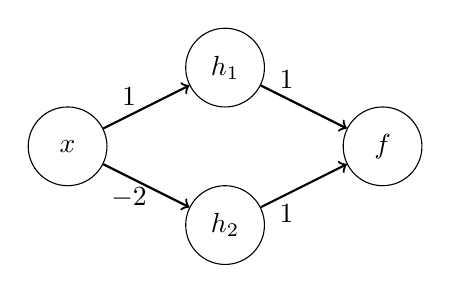
\begin{tikzpicture}[
                    neuron/.style={circle, draw=black, minimum size=1cm},
                    layer/.style={node distance=1.5cm and 2cm},
                    every edge/.style={draw,->,thick}
                ]

                % Input Layer
                \node[neuron] (I1) at (0,0) {$x$};

                \node[neuron] (H1) at (2, 1) {$h_1$};
                \node[neuron] (H2) at (2, -1) {$h_2$};

                % Output Layer
                \node[neuron] (O1) at (4, 0) {$f$};

                % Connections with weights
                \draw (I1) edge node[pos=0.3, above] {$1$} (H1);
                \draw (I1) edge node[pos=0.3, below] {$-2$} (H2);
                \draw (H1) edge node[pos=0.3, above] {$1$} (O1);
                \draw (H2) edge node[pos=0.3, below] {$1$} (O1);
            \end{tikzpicture}
            \captionof{figure}{Simple MLP using $\tanh(x)$ activation implementing a non-injective mapping.}
            \label{fig:non_injective_mlp_single_input}
        \end{center}

        \begin{center}
            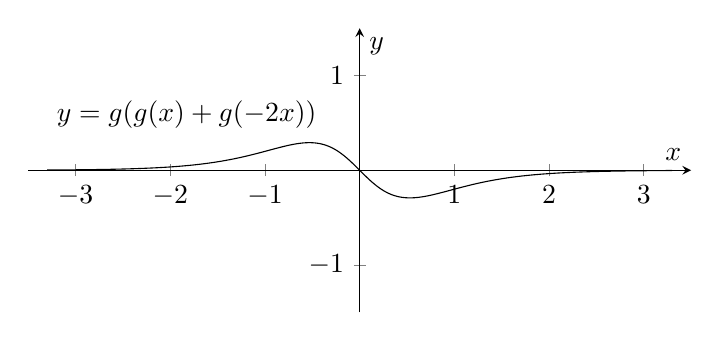
\begin{tikzpicture}[>=stealth]
                \begin{axis}[
                    axis equal image,
                    width=10cm,
                    xmin=-3.5,xmax=3.5,
                    ymin=-1.5,ymax=1.5,
                    axis x line=middle,
                    axis y line=middle,
                    axis line style=->,
                    xlabel={$x$},
                    ylabel={$y$},
                    ]
                    \addplot[no marks,black,-] expression[domain=-3.3:3.3,samples=1000]{tanh(tanh(x) + tanh(-2 * x))} 
                                node[pos=0,anchor=south west, yshift=0.4cm]{$y=g(g(x) + g(-2x))$}; 
                \end{axis}
            \end{tikzpicture}
            \captionof{figure}{Plot of the function $y=g(g(x) + g(-2x))$ with $g(x) \coloneqq \tanh(x)$.}
            \label{fig:non_injective_function}
        \end{center}
    \end{example}
\end{critique}

Regarding models that allocate more than one node per variable, Marcus states:

\begin{citecallout}[\textcite{marcus_algebraic_mind}]
    Models that allocate more than one node per variable too, can represent
    universally quantified one-to-one mappings (see, for example, the left
    panel of figure 3.4), but they do not have to (see the right panel of figure
    3.4).
\end{citecallout}

\begin{critique}
    This statement caries very little information. It only states that there exists MLPs that represent UQOTOMs, and that there exist MLPs that do not represent UQOTOMs, which is trivially true. The bigger problem, however, is that he also does not provide any further details on how to construct such MLPs, or what the implications of this distinction are.
\end{critique}

\subsubsection{Learning}
Until now, Marcus has only discussed the ability of MLPs to represent UQOTOMs. Now, he turns to the question of whether MLPs can \emph{learn} UQOTOMs. He states:

\begin{citecallout}[\textcite{marcus_algebraic_mind}]
    The flexibility in what multiple-nodes-per-variable models
    can represent leads to a flexibility in what they can learn. Multiple-
    nodes-per-variable models can learn UQOTOMs, and they can learn
    arbitrary mappings. But what they learn depends on the nature of the
    learning algorithm. Back-propagation—the learning algorithm most
    commonly used—does not allocate special status to UQOTOMs. Instead, a many-nodes-per-variable multilayer perceptron that is trained
    by back-propagation can learn a UQOTOM—such as identity, multiplication, or concatenation—only if it sees that UQOTOM illustrated with
    respect to each possible input and output node.
\end{citecallout}

He justifies that back-propagation does not allocate special status to UQOTOMs with an exapmle:

\begin{example}
    The autoencoder network depicted in \ref{fig:identity_autoencoder} is trained to learn the identity mapping:

    \begin{figure}[H]
        \centering
        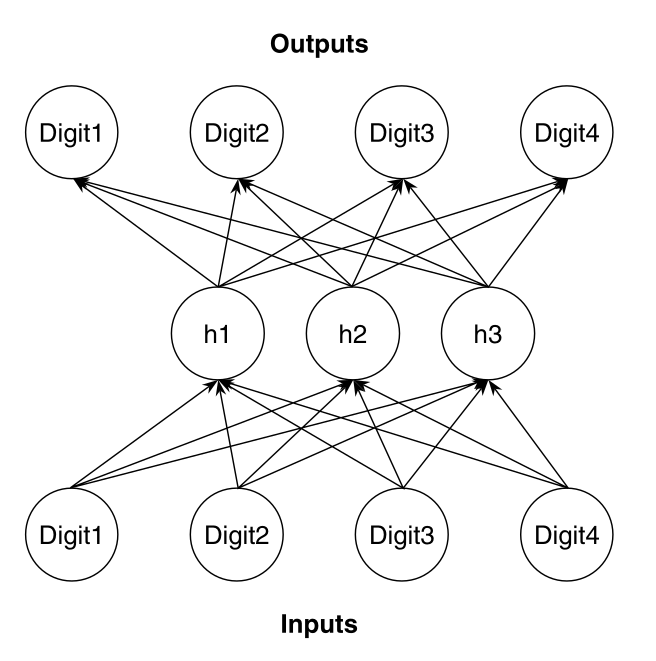
\includegraphics[width=0.5\textwidth]{chapters/relations_between_variables/network.png}
        \caption{Autoencoder network trained to learn the identity mapping.}
        \label{fig:identity_autoencoder}
    \end{figure}

    However, all training samples have a 0 as a last bit. Marcus' simulations show that the network learns to ignore the last bit by always predicting a 0, and only learns the identity mapping for the first three bits.
\end{example}

He formalizes this failure of back-propagation to learn UQOTOMs by defining the concept of \emph{training independence}:

\begin{citecallout}[\textcite{marcus_algebraic_mind}]
    The equations lead to two properties that I call input independence and
    output independence or, collectively, training independence (Marcus, 1998c).
\end{citecallout}

\begin{definition}[Input Independence]
    "\emph{Input independence is about how the connections that emanate from input nodes are trained. First, when an input node is always off (that is, set
    to 0), the connections that emanate from it will never change. This is
    because the term in the equation that determines the size of the weight
    change for a given connection from input node x into the rest of the network is always multiplied by the activation of input node x; if the activation of input node x is 0, the connection weight does not change.}" (Marcus, 2001, p. 47)
\end{definition}

\begin{definition}[Output Independence]
    "\emph{Output independence is about the connections that feed into the out-
    put units. The equations that adjust the weights feeding an output unit
    j depend on the difference between the observed output for unit j and
    the target output for unit j but not on the observed values or target values of
    any other unit. Thus the way the network adjusts the weights feeding out-
    put node j must be independent of the way the network adjusts the
    weights feeding output node k (assuming that nodes j and k are distinct).}" (Marcus, 2001, p. 47)
\end{definition}

\end{document}